\documentclass[11pt]{beamer}
\usetheme{Amsterdam}
\usepackage[utf8]{inputenc}
\usepackage{amsmath}
\usepackage{amsfonts}
\usepackage{amssymb}
\usepackage{hyperref}
\author{Callerisa \and Fontany-Legall \and Qui}
\title{Modélisation d'une colonie de fourmis}
%\setbeamercovered{transparent} 
%\setbeamertemplate{navigation symbols}{} 
%\logo{} 
\institute{Université de Nice} 
\date{\today} 
%\subject{} 
\begin{document}

\begin{frame}

\titlepage
\end{frame}
%\begin{frame}
%\tableofcontents
%\end{frame}

\begin{frame}
\frametitle{Colonie de fourmis}
\framesubtitle {Informations sur le modèle}
\begin{itemize}
\item Crée dans le cadre du projet "Connected mathematics: making sense of complex phenomena through building object-based parallel models"
\begin{itemize} 
\item Mise en relation des mathématiques avec d'autres domaines.
\item Analyse de phénomènes complexes grâce à des modèles multi-agents.
\end{itemize}
\item Développé en 1994 au MIT par Mitchel Resnik.
\end{itemize}
\end{frame}

\begin{frame}
\frametitle{Colonie de fourmis}
\framesubtitle{Recherche de nourriture}
\begin{block}{Modèle de base}
\begin{itemize}
\item fourmilière
\item tas de nourriture
\item fourmis (agents)
\end{itemize}
\end{block}
\begin{block}{Paramètres}
\begin{itemize}
\item Population
\item Taux de diffusion des phéromones
\item Vitesse d'évaporation des phéromones
\end{itemize}
\end{block}
\end{frame}

\begin{frame}
\frametitle{Démo}
\begin{figure}
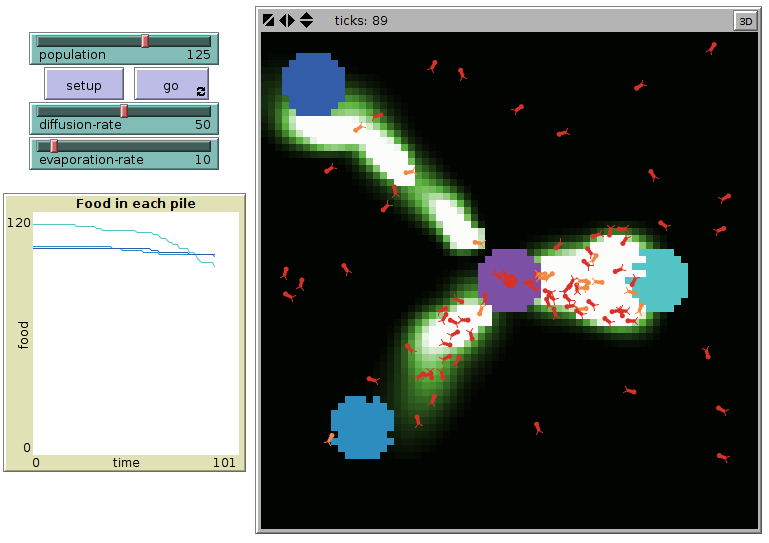
\includegraphics[scale=0.3]{Capture2.png}
\caption{Interface de la simulation}
\end{figure}
\end{frame}

\begin{frame}
\frametitle{Premières observations}
\begin{itemize}
\item Tendance à vider un tas de nourriture après l'autre avec les paramètres par défaut.
\item La diffusion et l'évaporation des phéromones sont nécessaires pour une récolte efficace.
\item Lorsque les phéromones ne persistent pas, tous les tas sont exploités en même temps et peu efficacement.
\end{itemize}
\end{frame}

\begin{frame}
\frametitle{Recherches préliminaires}
\begin{itemize}
\item Plusieurs manières de retrouver le nid
\begin{itemize}
\item Flair
\item Mémorisation de la distance et de la direction
\item Repères (visuels, olfactifs, tactiles)
\end{itemize}
\item Deux types de fourmis
\begin{itemize}
\item Chercheuses
\item Ramasseuses
\end{itemize}
\end{itemize}
\end{frame}

\begin{frame}
\frametitle{Objectifs}
\framesubtitle{Problématique}
\begin{center} De quelle manière les proportions de fourmis chercheuses et ramasseuses influent-elles sur la récolte de nourriture ?
\end{center}
\end{frame}

\begin{frame}

\frametitle{Objectifs}
\frametitle{Modèle envisagé}
\begin{block}{Hypothèses simplificatrices}
\begin{itemize}
\item Les fourmis retrouvent le chemin vers le nid au flair.
\item Le mouvement des fourmis qui ne suivent pas de phéromones est aléatoire.
\end{itemize}
\end{block}
\begin{block}{Améliorations du modèle de base}
\begin{itemize}
\item Création de fourmis chercheuses et ramasseuses.
\item Controle du nombre de fourmis de chaque type.
\item Possibilité de déplacer les tas de nourriture.
\end{itemize}
\end{block}
\end{frame}

\begin{frame}
\frametitle{Objectifs}
\framesubtitle{Tests envisagés}
\begin{itemize}
\item Variation des proportions des deux types de fourmis.
\item Variation de la distance de la nourriture.
\item Variation des phéromones.

\end{itemize}
\end{frame}

\begin{frame}
\frametitle{Credits}
\begin{itemize}
\item Wilensky, U. (1997). NetLogo Ants model. \url{http://ccl.northwestern.edu/netlogo/models/Ants}. Center for Connected Learning and Computer-Based Modeling, Northwestern University, Evanston, IL.
\item Wilensky, U. (1999). NetLogo. \url{http://ccl.northwestern.edu/netlogo/}. Center for Connected Learning and Computer-Based Modeling, Northwestern University, Evanston, IL.
\end{itemize}
\end{frame}

\begin{frame}
\frametitle{Credits}
\begin{itemize}
\item Liviu A. Panait and Sean Luke. (2004). \url{http://www.cc.gatech.edu/~turk/bio_sim/articles/ant_foraging_revisited.pdf} . George Mason University, Fairfax, VA 22030.
\end{itemize}
\end{frame}

\end{document}
